\documentclass[11pt]{article}
\usepackage[utf8]{inputenc}
\usepackage[T2A]{fontenc}
\usepackage[russian]{babel}
\usepackage{amsmath,amssymb}
\usepackage{graphicx}
\usepackage{authblk}
\usepackage{hyperref}
\graphicspath{{../../figures/}}
\newcommand{\keywords}[1]{\par\noindent\textbf{Ключевые слова:} #1}

\title{Адаптивный SPSA с моментом для оптимизации зашумлённых функций}
\author[1]{Иван Иванов}
\author[1]{Мария Петрова}
\author[1]{Елена Смирнова}
\affil[1]{Лаборатория стохастической оптимизации, Университет-Пример}

\begin{document}
\maketitle

\begin{abstract}
Исследуется стохастическая аппроксимация с одновременным возмущением (SPSA) с моментом при шуме измерений. На зашумлённой квадратичной функции размерности 10 момент $\beta = 0.6$ уменьшает итоговую квадратичную ошибку по сравнению с классическим SPSA при равном числе измерений.
\end{abstract}
\keywords{стохастическая аппроксимация, SPSA, момент, оптимизация с шумом}

\input{sections/intro}
\input{sections/methods}
\section{Результаты}\label{sec:results}
Стоит отметить, что в настоящее время метод SPSA играет ключевую роль в оптимизации; мы провели
серию экспериментов.
Момент -- в отличие от классической схемы -- сглаживает траекторию.
Метод не просто ускоряет сходимость, а делает её устойчивой к шуму --- это главный результат.
	Средняя ошибка после 300 итераций показана на рисунке.
\begin{equation}
E
=
\frac{1}{N}
\sum_i
\|x_i\|^2
\end{equation}
\begin{figure}[t]
\centering
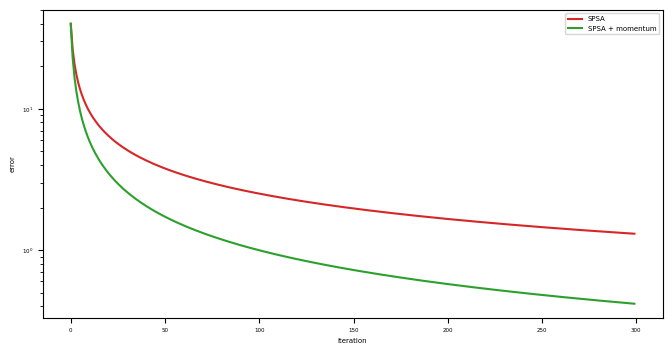
\includegraphics[width=\linewidth]{convergence_bad.png}
\caption{Сходимость SPSA и SPSA с моментом.}
\end{figure}

\input{sections/discussion}
\input{sections/conclusion}

\section*{Доступность данных}
Код и данные доступны в репозитории проекта.

\section*{Финансирование}
Не применимо.

\section*{Конфликт интересов}
Авторы заявляют об отсутствии конфликта интересов.

\section*{Вклад авторов}
Все авторы внесли равный вклад.

\section*{Использование генеративного ИИ}
Генеративный ИИ при написании текста не использовался.

\bibliographystyle{unsrt}
\bibliography{../references}
\end{document}
